\newpage
\section{Experiment 5 - Interpretability Objective}
\label{sec:exp5}
When looking back on the solution with an optimal fitness found in one of the experiments in Experiment 2, it can be noted that the matrix decomposition of the resulting UPA (see Figure \ref{fig:exp2b_RM}) looks different than the matrices dataset 1 has been constructed on (see Figure \ref{fig:dataset1}). It shows that several solutions for a matrix decomposition can exist. To distinguish them another measure is needed. 

One reason why bottom-up role mining is criticized, is that a solution might be found based on given technical data (user-permission-assignments), but it is not necessary feasible for the business. Therefore the Interpretability objective and the fitness functions
$F_{basic\_INT}^{min}$ \eqref{eq:FEdgeMin_INT} and $F_{edge\_INT}^{min}$ \eqref{eq:FEdgeMin_INT} are observed in this phase.

For the experiments the setup in table \ref{tab:exp3_setup} is taken and executed on the Dataset1. The weight for the interpretability measure is set 1.0. The results can be seen in Figure \ref{fig:Results_Exp5}.

\begin{figure}[H]
	\centering
	\begin{subfigure}{0.45\textwidth}
		%\centering
		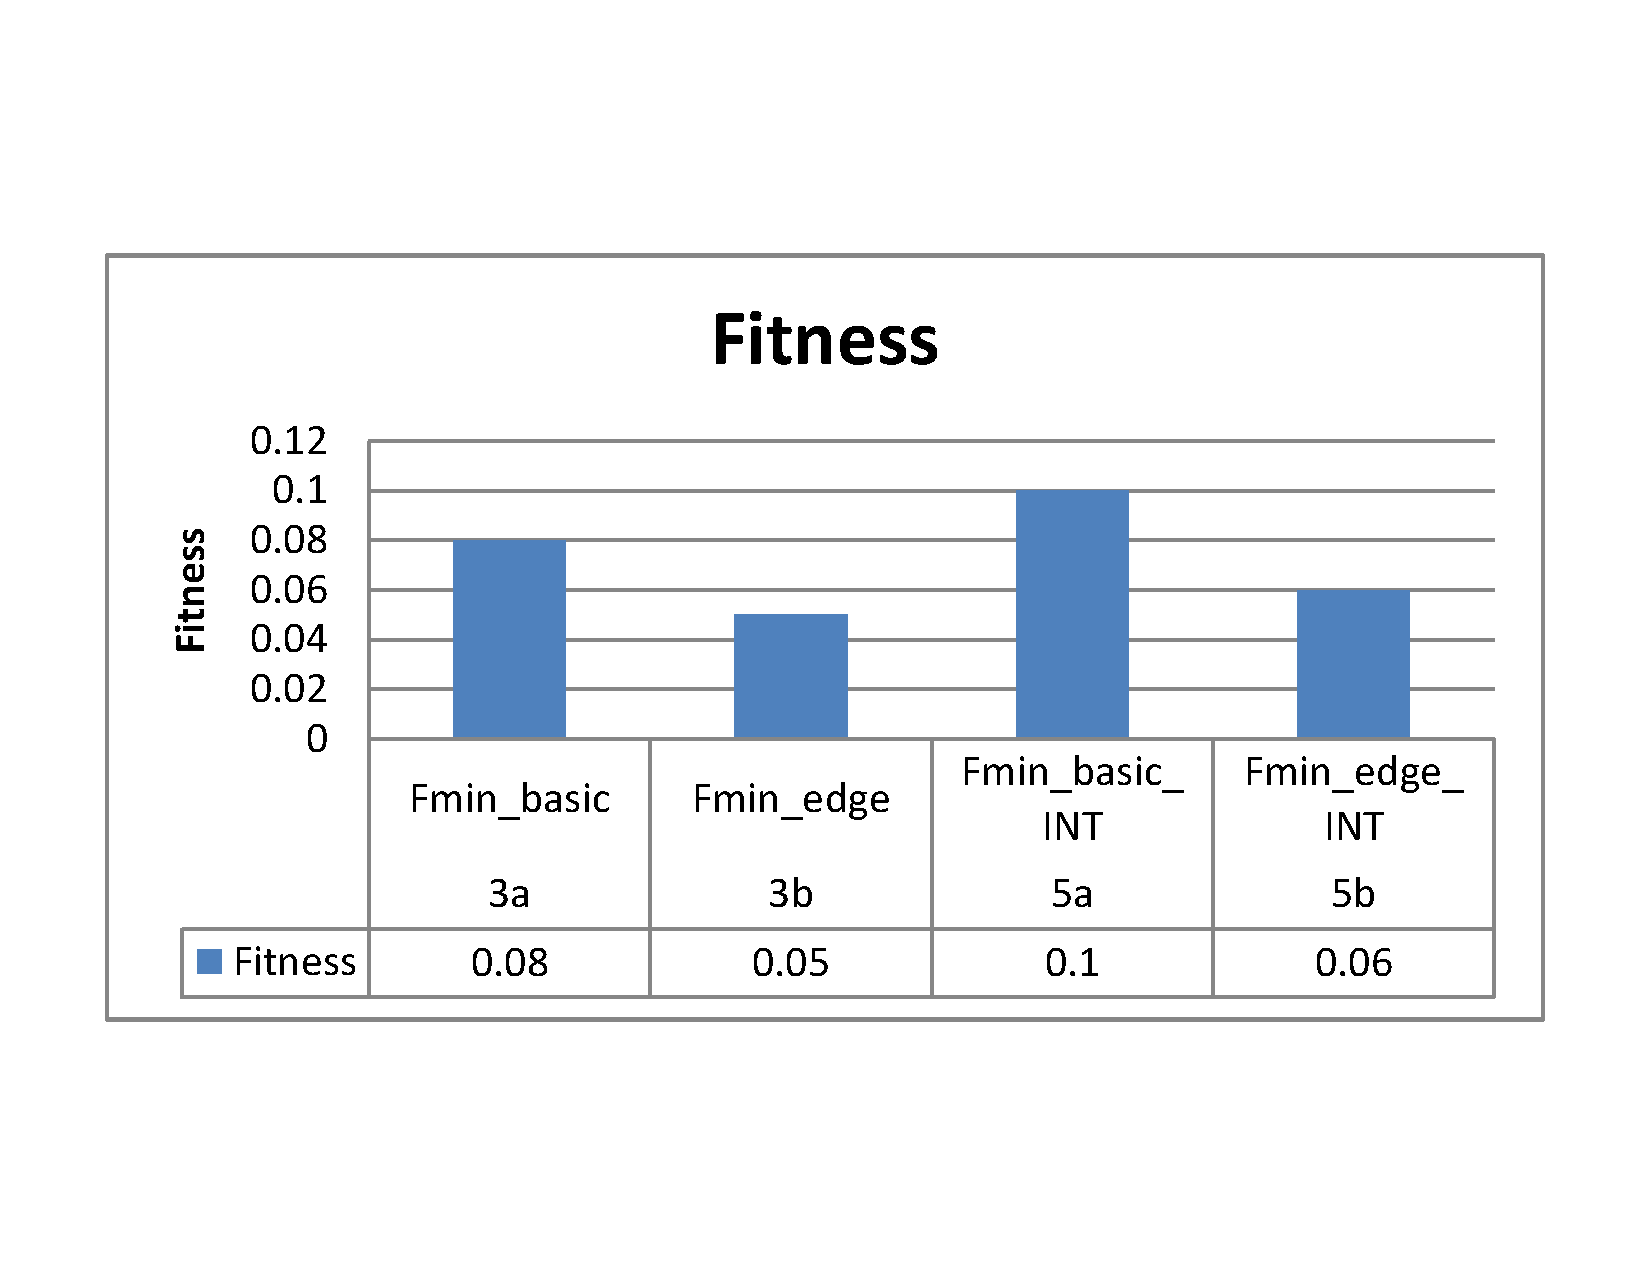
\includegraphics[width=\textwidth, trim=1cm 2cm 1cm 1.5cm, clip=true]{Results_Exp5_Dataset1_Fitness}
		\caption{Dataset1}
		\label{fig:Results_Exp5_Dataset1_Fitness}
	\end{subfigure}%
	\begin{subfigure}{0.55\textwidth}
		\centering
		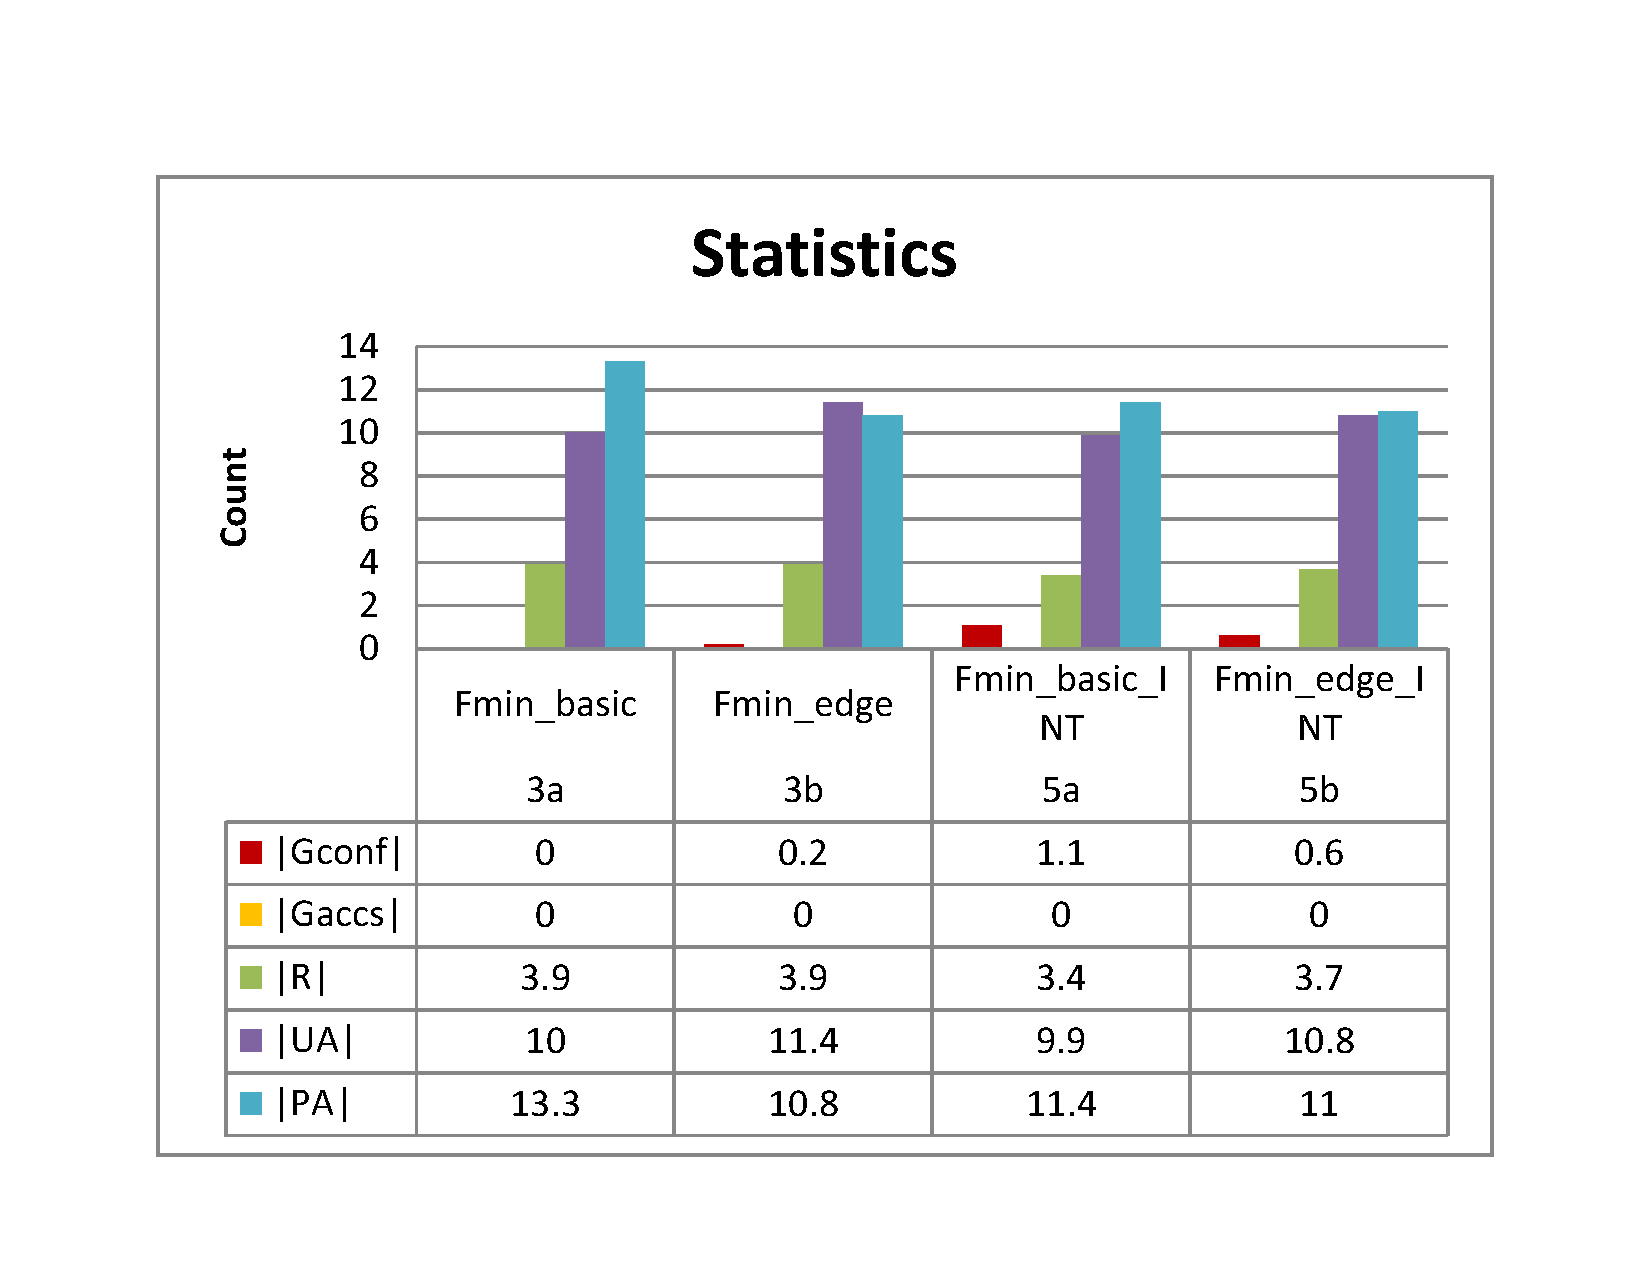
\includegraphics[width=\textwidth, trim=2cm 2cm 2cm 1.5cm, clip=true]{Results_Exp5_Dataset1_Statistics}
		\caption{Dataset1}
		\label{fig:Results_Exp5_Dataset1_Statistics}
	\end{subfigure}
	\caption{EXPERIMENT5: Statistics of ten experiments with the Evo-RoleMiner with setup in Table \ref{tab:exp2_setup} for Dataset1. The values for Fitness, Confidentiality violations ($|G_{conf}|$), Availability violations ($|G_{accs}|$), Roles ($|R|$), User-Role-Assignments ($|UA|$) and Role-Permission assignments ($|PA|$) are the average minimum in the last Generation of all experiments.}
	\label{fig:Results_Exp5}
\end{figure}

The same experiments have been executed on the healthcare dataset with the user attribute information provided by Xu \& Stoller\cite{Xu}. The experiments have been aborted after the fitness calculation of the first generation could not be finished in a decent time. There are 20 attributes for the users in the healthcare dataset. For the interpretability measure rules are generated, where $2^X-1$ combinations of X attributes are created. While for Dataset1 with 3 user attributes seven combinations are created and tested, the healthcare dataset requires 1048575 combinations for 20 attributes. The rule induction gets too expensive to finish in reasonable time.